% ====================================
\chapter{Les tableaux à 2 dimensions}
% ====================================

% ===================
\section{Définition}
% ===================

	\marginicon{definition}
	La \textbf{dimension} d’un tableau est le nombre d’indices qu’on utilise
	pour faire référence à un de ses éléments. Attention de ne pas confondre 
	avec la	taille !
	
	En \abbr{dev1}, nous avons introduit les tableaux à une dimension.
	Un seul indice suffisait à localiser un de ses éléments. 
	Pour le dire autrement,
	chaque case possédait \textbf{un} numéro.
	De nombreuses situations nécessitent cependant l’usage de tableaux à deux dimensions.
	Ils vous sont déjà familiers par leur présence dans beaucoup de
	situations courantes : calendrier, grille horaire, grille de mots
	croisés, sudoku, jeux se déroulant sur un quadrillage (damier,
	échiquier, scrabble\dots).
	Dans ces situations, 
	chaque case est désignée par \textbf{deux} numéros.

% ====================
\section{Notations}
% ====================

	\subsection{Déclarer}
	%====================
		
		\marginicon{definition}
		Pour \textbf{déclarer} un tableau à 2 dimensions, on écrira :
	
		\begin{algo}
			\Decl{nomTableau}{\Array{nbLignes $\times$ nbColonnes}{TypeElément}}\;
		\end{algo}
	
		où \lda{nbLignes} et \lda{nbColonnes} 
		sont des expressions entières quelconques.
	
		\textbf{Exemple} :
		
		\begin{algo}
			\Decl{tab}{\Array{5$\times$10}{integers}}\;
		\end{algo}
		
		déclare un tableau de 5 lignes par 10 colonnes dont chaque case
		contient un entier.
		
	\subsection{Utiliser}
	%====================

		\marginicon{definition}
		Pour \textbf{accéder} à une case du tableau on donnera les deux indices
		entre crochets.
		Comme en \abbr{dev1}, on considère que la première ligne 
		et la première colonne portent le numéro (l'indice) $0$.  
		
		\textbf{Exemple} :
		
		\begin{algo}
			\Write tab[2,4]
				\RComment{affiche le 5\ieme{} élément de la 3\ieme{} ligne du tableau nommé \samp{tab}.}
		\end{algo}
		
	\subsection{Visualiser}
	%======================

		Notez que la vue sous forme de tableau avec des lignes
		et des colonnes est une vision humaine.
		Il n'y a pas de lignes ni de colonnes en mémoire.
		Pour être précis,
		on devrait juste parler de première dimension et
		de deuxième dimension
		mais la notion de ligne et de colonne
		est un abus de langage qui simplifie le discours.
		
		On pourrait aussi visualiser un tableau à deux dimensions
		comme un tableau à une dimension dont chacun des éléments est
		lui-même un tableau à une dimension.
	
		\textbf{Exemple} : Soit le tableau déclaré ainsi :
	
		\begin{algo}
		\Decl{nombres}{\Array{4$\times$5}{integers}}\;
		\end{algo}
	
		On peut le visualiser à l’aide d’une grille à 4 lignes et 5 colonnes.

		\begin{center}
		\begin{tabular}{*{6}{>{\centering\arraybackslash}m{5mm}}}
			{} & 0 & 1 & 2 & 3 & 4 \\
		\end{tabular}
		\\
		\begin{tabular}{>{\centering\arraybackslash}m{3mm}|*{5}{>{\centering\arraybackslash}m{5mm}|}}
			\cline{2-6}
			0 & 0 & 1 & 2 & 3 & 4 \\\cline{2-6}
			1 & 10 & 11 & 12 & 13 & 14 \\\cline{2-6}
			2 & 20 & 21 & 22 & 23 & 24 \\\cline{2-6}
			3 & 30 & 31 & 32 & 33 & 34 \\\cline{2-6}
		\end{tabular}
		\end{center}
	
		Ainsi, la valeur de \lda{nombres[2,3]} 
		est la valeur 23. 
		
		La vision «~tableau de tableaux~» 
		(ou décomposition en niveaux)
		donnerait :
	
		\begin{center}
		\begin{tabular}{*{4}{>{\centering\arraybackslash}m{30mm}}}
			0 & 1 & 2 & 3 \\
		\end{tabular}
		\\
		\begin{tabular}{|*{4}{>{\centering\arraybackslash}m{30mm}|}}
			\hline
			\begin{minipage}{30mm}
				\begin{tabular}{*{5}{>{\centering\arraybackslash}m{1.5mm}}}
					0 & 1 & 2 & 3 & 4 \\
				\end{tabular}
				\\		
				\begin{tabular}{|*{5}{>{\centering\arraybackslash}m{1.5mm}|}}
					\hline
					0 & 1 & 2 & 3 & 4 \\
					\hline
				\end{tabular}
				\\
			\end{minipage}
			& 
			\begin{minipage}{30mm}
				\begin{tabular}{*{5}{>{\centering\arraybackslash}m{1.5mm}}}
					0 & 1 & 2 & 3 & 4 \\
				\end{tabular}
				\\		
				\begin{tabular}{|*{5}{>{\centering\arraybackslash}m{1.5mm}|}}
					\hline
					10 & 11 & 12 & 13 & 14 \\
					\hline
				\end{tabular}
				\\
			\end{minipage}
			& 
			\begin{minipage}{30mm}
				\begin{tabular}{*{5}{>{\centering\arraybackslash}m{1.5mm}}}
					0 & 1 & 2 & 3 & 4 \\
				\end{tabular}
				\\		
				\begin{tabular}{|*{5}{>{\centering\arraybackslash}m{1.5mm}|}}
					\hline
					20 & 21 & 22 & 23 & 24 \\
					\hline
				\end{tabular}
				\\
			\end{minipage}
			& 
			\begin{minipage}{30mm}
				\begin{tabular}{*{5}{>{\centering\arraybackslash}m{1.5mm}}}
					0 & 1 & 2 & 3 & 4 \\
				\end{tabular}
				\\		
				\begin{tabular}{|*{5}{>{\centering\arraybackslash}m{1.5mm}|}}
					\hline
					30 & 31 & 32 & 33 & 34 \\
					\hline
				\end{tabular}
				\\
			\end{minipage}
			\\
			\hline
		\end{tabular}
		\end{center}

		Dans cette représentation, le tableau \lda{nombres} est
		d’abord décomposé à un premier niveau en quatre éléments auxquels on
		accède par le premier indice. Ensuite, chaque élément de premier niveau
		est décomposé en cinq éléments de deuxième niveau accessibles par le
		deuxième indice.

	\subsection{Exemples}
	%======================
	
		\paragraph{Exemple 1 -- Remplir les coins.}
		Dans ce petit exemple,
		on a un tableau de chaines et on donne des valeurs aux coins.
		
		\begin{center}
			\begin{tabular}{|*{5}{>{\centering\arraybackslash}m{1cm}|}}
				\hline
				"NO" &
				 &
				 &
				 &
				"NE"
				\\\hline
				 &
				 &
				 &
				 &
				\\\hline
				"SO" &
				 &
				 &
				 &
				"SE"
				\\\hline
			\end{tabular}	
		\end{center}
		
		\begin{algo}
		\Comment{Déclare un tableau et donne des valeurs aux coins.}\;
		\Algo{remplirCoins}{}{}{
			\Decl{grille}{\Array{3$\times$5}{string}}\;
			grille[0,0] \Gets "NO"\;
			grille[0,4] \Gets "NE"\;
			grille[2,0] \Gets "SO"\;
			grille[2,4] \Gets "SE"\;
		}
		\end{algo}
	
		\newpage
		La version \bsc{Java} :
		\listing*[linerange=11-18]{java}{java/src/main/java/dev2/algo/tab/Exemple1.java}
		
		\paragraph{Exemple 2 -- Gestion des stocks.}
		Reprenons l'exemple du stock de 10 produits
		qui a servi d'introduction au chapitre sur les tableaux
		mais, cette fois, pour chaque jour de la semaine.
	
		\begin{small}
		\begin{center}
			%\begin{tabular}{*{8}{>{\centering\arraybackslash}m{1.2cm}}}
			\begin{tabular}{m{1.5cm}*{7}{>{\centering\arraybackslash}m{1.2cm}}}
				~ & {article0} & {article1} & {article2} & \dots & {article7} & {article8} & {article9}\\
			\end{tabular}	
			\begin{tabular}{|m{1.5cm}|*{7}{>{\centering\arraybackslash}m{1.2cm}|}}
				\hline
				{lundi}    & {cpt[0,0]} & {cpt[0,1]} & {cpt[0,2]} & \dots & {cpt[0,7]} & {cpt[0,8]} & {cpt[0,9]} \\\hline
				{mardi}    & {cpt[1,0]} & {cpt[1,1]} & {cpt[1,2]} & \dots & {cpt[1,7]} & {cpt[1,8]} & {cpt[1,9]} \\\hline
				{mercredi} & {cpt[2,0]} & {cpt[2,1]} & {cpt[2,2]} & \dots & {cpt[2,7]} & {cpt[2,8]} & {cpt[2,9]} \\\hline
				{jeudi}    & {cpt[3,0]} & {cpt[3,1]} & {cpt[3,2]} & \dots & {cpt[3,7]} & {cpt[3,8]} & {cpt[3,9]} \\\hline
				{vendredi} & {cpt[4,0]} & {cpt[4,1]} & {cpt[4,2]} & \dots & {cpt[4,7]} & {cpt[4,8]} & {cpt[4,9]} \\\hline
				{samedi}   & {cpt[5,0]} & {cpt[5,1]} & {cpt[5,2]} & \dots & {cpt[5,7]} & {cpt[5,8]} & {cpt[5,9]} \\\hline
				{dimanche} & {cpt[6,0]} & {cpt[6,1]} & {cpt[6,2]} & \dots & {cpt[6,7]} & {cpt[6,8]} & {cpt[6,9]} \\\hline
			\end{tabular}
		\end{center}
		\end{small}
		
		\bigskip
		
		\begin{algo}
		\Comment{Calcule et affiche la quantité vendue de 10 produits}\;
		\Comment{pour chaque jour de la semaine (de 0~: lundi à 6~: dimanche).}\;
		\Algo{statistiquesVentesSemaine}{}{}{
			\Decl{cpt}{\Array{7$\times$10}{integers}}\;
			initialiser(cpt)\;
			\Fori{jour}{0}{6\hfill\Comment{Pour chaque jour de la semaine}}{
				\Write "jour: ", jour
				traiterStock1Jour(cpt, jour)\;
				\Fori{produit}{0}{9}{
					\Write "quantité vendue de produit ", produit, 
					" ce jour ", jour, "~: ", cpt[jour,produit]\;
				}
			}
		}
		\end{algo}
	
		\begin{algo}
		\Comment{Initialise le tableau d'entiers à 0}\;
		\Algo{initialiser}{\Par{entiers\InOut}{\Array{7$\times$10}{integers}}}{}{
			\Fori{i}{0}{6}{
				\Fori{j}{0}{9}{
					entiers[i,j] \Gets 0\;
				}
			}
		}
		\end{algo}
	
		\begin{algo}
		\Comment{Effectue le traitement du stock pour une journée.}\;
		\Algo{traiterStock1Jour}{\Par{cpt\InOut}{\Array{7$\times$10}{integers}}, \Par{jour\In}{integer}}{}{
			\Decl{numéroProduit, quantité}{integers}\;
			numéroProduit \Gets \Ask{"Introduisez le numéro du produit~:"}\; 
			\While{numéroProduit $\geq$ 0 et numéroProduit $<$ 10}{
				quantité \Gets \Ask{"Introduisez la quantité vendue~:"}\;
				cpt[jour,numéroProduit] \Gets cpt[jour,numéroProduit] + quantité\;
				numéroProduit \Gets \Ask{"Introduisez le numéro du produit~:"}\;
			}
		}
		\end{algo}
	
		\newpage
		En \bsc{Java} :
		\listing*[linerange=11-37]{java}{java/src/main/java/dev2/algo/tab/Exemple2.java}

	\subsection{Exercices}
			
		\begin{Exercice}{Case nulle ?}
			Écrire un algorithme qui reçoit un tableau d'entiers
			(à $n$ lignes et $m$ colonnes)
			ainsi que les coordonnées d'une case (ligne, colonne)
			et qui retourne un booléen indiquant si la case désignée
			contient ou pas la valeur nulle.
			
			\begin{algo}
				\AlgoSign{estNul}{\Par{tab}{\Array{n $\times$ m}{integers}}, \Par{lg, col}{integers}}{boolean}\;
			\end{algo}
		\end{Exercice}

		\begin{Solution}
			\begin{algo}
				\Algo{estNul}{\Par{tab}{\Array{n $\times$ m}{integers}}, \Par{lg, col}{integers}}{boolean}{
					\Return tab[lg][col]=0\;
				}
			\end{algo}
		\end{Solution}

		\begin{Exercice}{Assigner une case}
			Écrire un algorithme qui reçoit un tableau d'entiers
			(à $n$ lignes et $m$ colonnes)
			ainsi que les coordonnées d'une case (ligne, colonne)
			et une valeur entière.
			L'algorithme met la valeur donnée dans la case indiquée
			pour autant que la case contienne actuellement la valeur nulle.
			Dans le cas contraire, l'algorithme ne fait rien.
			
			\begin{algo}
				\AlgoSign{assigner}{\Par{tab\InOut}{\Array{n $\times$ m}{integers}}, \Par{lg\In, col\In, val\In}{integers}}{}\;
			\end{algo}
		\end{Exercice}

		\begin{Solution}
			\begin{algo}
				\Algo{assigner}{\Par{tab\InOut}{\Array{n $\times$ m}{integers}}, \Par{lg\In, col\In, val\In}{integers}}{}{
					\If{estNul(tab, lg, col)}{
						tab[lg,col] \Gets val\;
					}
				}
			\end{algo}
		\end{Solution}

		\begin{Exercice}{Un bord du tableau}
			Écrire un algorithme qui reçoit un tableau d'entiers
			(à $n$ lignes et $m$ colonnes)
			ainsi que les coordonnées d'une case (ligne, colonne).
			L'algorithme doit indiquer si la case donnée
			est ou non sur un \textbf{bord} du tableau.
			
			\begin{algo}
				\AlgoSign{estBord}{\Par{tab}{\Array{n $\times$ m}{integers}}, \Par{lg, col}{integers}}{boolean}\;
			\end{algo}
		\end{Exercice}

		\begin{Solution}
			\begin{algo}
				\Algo{estBordHaut}{\Par{tab}{\Array{n$\times$m}{entiers}}, \Par{lg, col}{entiers}}{booléen}{
					\Return lg = 0
				}
				\BlankLine
				\Algo{estBordBas}{\Par{tab}{\Array{n$\times$m}{entiers}}, \Par{lg, col}{entiers}}{booléen}{
					\Return lg = n - 1
				}
				\BlankLine
				\Algo{estBordGauche}{\Par{tab}{\Array{n$\times$m}{entiers}}, \Par{lg, col}{entiers}}{booléen}{
					\Return col = 0
				}
				\BlankLine
				\Algo{estBordDroit}{\Par{tab}{\Array{n$\times$m}{entiers}}, \Par{lg, col}{entiers}}{booléen}{
					\Return col = m - 1
				}
				\BlankLine
				\Algo{estBord}{\Par{tab}{\Array{n$\times$m}{entiers}}, \Par{lg, col}{entiers}}{booléen}{
					\Return estBordGauche(tab,lg,col) OU estBordDroit(tab,lg,col)\;
						\Indp OU estBordHaut(tab,lg,col) OU estBordBas(tab,lg,col)\;
				}
			\end{algo}
		\end{Solution}

		\begin{Exercice}{Un coin du tableau}
			Écrire un algorithme qui reçoit un tableau d'entiers
			(à $n$ lignes et $m$ colonnes)
			ainsi que les coordonnées d'une case (ligne, colonne).
			L'algorithme doit indiquer si la case donnée
			est ou non sur un des 4 \textbf{coins} du tableau.
			
			\begin{algo}
				\AlgoSign{estCoin}{\Par{tab}{\Array{n $\times$ m}{integers}}, \Par{lg, col}{integers}}{boolean}\;
			\end{algo}
		\end{Exercice}

		\begin{Solution}
			\begin{algo}
				\Algo{estCoinHG}{\Par{tab}{\Array{n$\times$m}{entiers}}, \Par{lg, col}{entiers}}{booléen}{
					\Return estBordGauche(tab, lg, col) ET estBordHaut(tab, lg, col)
				}
				\BlankLine
				\Algo{estCoinHD}{\Par{tab}{\Array{n$\times$m}{entiers}}, \Par{lg, col}{entiers}}{booléen}{
					\Return estBordDroit(tab, lg, col) ET estBordHaut(tab, lg, col)
				}
				\BlankLine
				\Algo{estCoinBG}{\Par{tab}{\Array{n$\times$m}{entiers}}, \Par{lg, col}{entiers}}{booléen}{
					\Return estBordGauche(tab, lg, col) ET estBordBas(tab, lg, col)
				}
				\BlankLine
				\Algo{estCoinBD}{\Par{tab}{\Array{n$\times$m}{entiers}}, \Par{lg, col}{entiers}}{booléen}{
					\Return estBordDroit(tab, lg, col) ET estBordBas(tab, lg, col)
				}
				\BlankLine
				\Algo{estCoin}{\Par{tab}{\Array{n$\times$m}{entiers}}, \Par{lg, col}{entiers}}{booléen}{
					\Return estCoinHG(tab,lg,col) OU estCoinHD(tab,lg,col)\;
						\Indp OU estCoinBG(tab,lg,col) OU estCoinBD(tab,lg,col)\;
				}
			\end{algo}
		\end{Solution}

% ============================================
\section{La troisième dimension (et au-delà)}
% ============================================

	Certaines situations complexes nécessitent l'usage de
	tableaux à 3 voire plus de dimensions.

	\marginicon{definition}
	Pour déclarer un tableau statique à $k$ dimensions, on écrira :

	\begin{algo}
	\Decl{nomTableau}{\Array{tailleDim1 $\times$ \dots{} $\times$ tailleDimK}{TypeElément}}\;
	\end{algo}
	
% ================================================
\section{Parcours d'un tableau à deux dimensions}
\label{algo:Tab2D}
% ================================================

	Comme nous l'avons fait pour les tableaux à  une dimension,
	envisageons le parcours des tableaux à deux dimensions 
	($n$ lignes et $m$ colonnes).
	Nos algorithmes sont valables quel que soit le type des éléments.
	Utilisons \lda{T}%
	\footnote{%
		Nos versions \bsc{Java} seront écrits avec des tableau d'entiers.
		Il est possible de les écrire avec un type \emph{générique} \lda{T}
		mais ça requiert des notions avancées de \bsc{Java}.
	} pour désigner un type quelconque.
	
	\begin{algo}
		\Decl{tab}{\Array{n $\times$ m}{T}}\;
	\end{algo}
	
	Commençons par des cas plus simples 
	où on ne parcourt qu'une seule des dimensions 
	puis attaquons le cas général.

	\subsection{Parcours d'une dimension}
	%====================================
	
		Certains parcours ne visitent qu'une partie du tableau
		et ne nécessitent qu'une seule boucle.
		Examinons quelques cas.

		\paragraph{Une ligne.}
		On peut vouloir ne parcourir qu'une seule ligne du tableau.
		Si on parcourt la ligne $l$, on visite les cases 
		$(l,0)$, $(l,1)$, \dots, $(l,m-1)$.
		L'indice de ligne est constant et c'est l'indice de colonne qui varie.
		
		\begin{center}
		$l$
		\begin{tabular}{|*{5}{>{\centering\arraybackslash}m{0.3cm}|}}
		\hline
		\ & \ & \ & \ & \  \\
		\hline
		\cellcolor{gray!25}1 & \cellcolor{gray!25}2 & \cellcolor{gray!25}3 & \cellcolor{gray!25}4 & \cellcolor{gray!25}5  \\
		\hline
		\ & \ & \ & \ & \  \\
		\hline
		\end{tabular}
		\end{center}
		
		Ce qui donne l'algorithme :

		\begin{algo}
			\Comment{Parcours de la ligne $lg$ d'un tableau à deux dimensions}\;
			\Algo{afficherLigne}{%
                          \Par{tab}{\Array{n $\times$ m}{T}},
                          \Par{lg}{integer}}{}
                        {
				\ForAll{col : numéro de colonne \Comment{Pour tous les numéros de colonne}}{
					\Write tab[ lg, col ] \RComment{On peut faire autre chose qu'afficher}
				}
			}
		\end{algo}

		% \begin{algo}
		% 	\Comment{Parcours de la ligne $ligne$ d'un tableau à deux dimensions}\;
		% 	\Algo{afficherLigne}{%
        %                   \Par{tab}{\Array{n $\times$ m}{T}},
        %                   \Par{ligne}{integer}}{}
        %                 {
		% 		\Fori{colonne}{0}{m-1}{
		% 			\Write tab[ligne,colonne] \RComment{On peut faire autre chose qu'afficher}
		% 		}
		% 	}
		% \end{algo}

		\listing*[linerange=9-13]{java}{java/src/main/java/dev2/algo/tab/Parcours1D.java}

		\medskip
		\begin{infotbox}{Retenons}
			Pour parcourir une ligne, on utilise une boucle sur les colonnes. 
		\end{infotbox}

		\paragraph{Une colonne.}
		Symétriquement, on pourrait considérer le parcours d'une colonne
		avec l'algorithme suivant.
		
		\begin{algo}
			\Comment{Parcours de la colonne $col$ d'un tableau à deux dimensions}\;
			\Algo{afficherColonne}{\Par{tab}{\Array{n $\times$ m}{T}}, 
				\Par{col}{integer}}{}{
				\ForAll{lg : numéro de ligne \Comment{Pour tous les numéros de ligne}}{
					\Write tab[ lg, col ] \RComment{On peut faire autre chose qu'afficher}
				}
			}
		\end{algo}

		% \begin{algo}
		% 	\Comment{Parcours de la colonne $colonne$ d'un tableau à deux dimensions}\;
		% 	\Algo{afficherColonne}{\Par{tab}{\Array{n $\times$ m}{T}}, 
		% 		\Par{colonne}{integer}}{}{
		% 		\Fori{ligne}{0}{n-1}{
		% 			\Write tab[ligne,colonne] \RComment{On peut faire autre chose qu'afficher}
		% 		}
		% 	}
		% \end{algo}

		\listing*[linerange=15-19]{java}{java/src/main/java/dev2/algo/tab/Parcours1D.java}

		\paragraph{La diagonale descendante.}
		Si le tableau est carré ($n=m$) on peut aussi envisager le parcours
		des deux diagonales.
		
		Pour la diagonale descendante, 
		les éléments à visiter sont $(0,0)$, $(1,1)$, $(2,2)$, \dots, $(n-1,n-1)$.
		
		\begin{center}
		\begin{tabular}{|*{3}{>{\centering\arraybackslash}m{0.3cm}|}}
		\hline
		\cellcolor{gray!25}1 & \ & \ \\
		\hline
		\ & \cellcolor{gray!25}2 & \ \\
		\hline
		\ & \ & \cellcolor{gray!25}3 \\
		\hline
		\end{tabular}
		\end{center}
		
		Une seule boucle suffit 
		comme le montre l'algorithme suivant.
		
		\begin{algo}
			\Comment{Parcours de la diagonale descendante d'un tableau carré}\;
			\Algo{afficherDiagonaleDescendante}{\Par{tab}{\Array{n $\times$ n}{T}}}{}{
				\Fori{i}{0}{n-1}{
					\Write tab[i,i] \RComment{On peut faire autre chose qu'afficher}
				}
			}
		\end{algo}

		\listing*[linerange=21-25]{java}{java/src/main/java/dev2/algo/tab/Parcours1D.java}

		\paragraph{La diagonale montante.}
		Pour la diagonale montante, 
		on peut envisager deux solutions, 
		avec deux indices ou un seul
		en se basant sur le fait que 
		$\mathit{lg}+\mathit{col}=n-1 \Rightarrow \mathit{col}=n-1-\mathit{lg}$.
		
		\begin{center}
		\begin{tabular}{|*{3}{>{\centering\arraybackslash}m{0.3cm}|}}
		\hline
		\ & \ & \cellcolor{gray!25}1 \\
		\hline
		\ & \cellcolor{gray!25}2 & \ \\
		\hline
		\cellcolor{gray!25}3 & \ & \ \\
		\hline
		\end{tabular}
		\end{center}
		
		\begin{algo}
		\Comment{Parcours de la diagonale montante d'un tableau carré - version 2 indices}\;
		\Comment{lg part du début et augmente / col part de la fin et diminue}\;
		\Algo{afficherDiagonaleMontante}{\Par{tab}{\Array{n $\times$ n}{T}}}{}{
			\Decl{col}{integer}\;
			col \Gets n-1\;
			\Fori{lg}{0}{n-1}{
				\Write tab[ lg, col ] \RComment{On peut faire autre chose qu'afficher}
				col \Gets col - 1\;
			}
		}
		\end{algo}
		
		\begin{algo}
		\Comment{Parcours de la diagonale montante d'un tableau carré - version 1 indice}\;
		\Algo{afficherDiagonaleMontante}{\Par{tab}{\Array{n $\times$ n}{T}}}{}{
			\Fori{lg}{0}{n-1}{
				\Write tab[ lg, n-1-lg ]  \RComment{On peut faire autre chose qu'afficher}
			}
		}
		\end{algo}

		\listing*[linerange=27-48]{java}{java/src/main/java/dev2/algo/tab/Parcours1D.java}

	\subsection{Parcours des deux dimensions}
	%========================================
	
		\paragraph{Parcours par lignes et par colonnes.}
		%---------------------------------------------------
			
			Les deux parcours les plus courants sont les parcours ligne par ligne
			et colonne par colonne.
			Les tableaux suivants montrent dans quel ordre chaque case est visitée dans ces deux parcours.
			
			\begin{center}
			\begin{minipage}{0.4\textwidth}
			\begin{center}
			Parcours ligne par ligne\\
			\begin{tabular}{|*{5}{>{\centering\arraybackslash}m{0.35cm}|}}
			\hline
			1 & 2 & 3 & 4 & 5 \\
			\hline
			6 & 7 & 8 & 9 & 10 \\
			\hline
			11 & 12 & 13 & 14 & 15 \\
			\hline
			\end{tabular}
			\end{center}
			\end{minipage}
			\qquad
			\begin{minipage}{0.4\textwidth}
			\begin{center}
			Parcours colonne par colonne\\
			\begin{tabular}{|*{5}{>{\centering\arraybackslash}m{0.35cm}|}}
			\hline
			1 & 4 & 7 & 10 & 13 \\
			\hline
			2 & 5 & 8 & 11 & 14 \\
			\hline
			3 & 6 & 9 & 12 & 15 \\
			\hline
			\end{tabular}
			\end{center}
			\end{minipage}
			\end{center}
			
			Le plus simple est d'utiliser deux boucles imbriquées 
			
			\begin{algo}
			\Comment{Parcours d'un tableau à 2 dimensions, ligne par ligne}\;
			\Algo{afficherLigneParLigne}{\Par{tab}{\Array{n $\times$ m}{T}}}{}{
				\Fori{lg}{0}{n-1}{
					\Fori{col}{0}{m-1}{
						\Write tab[lg,col] \RComment{On peut faire autre chose qu'afficher}
					}
				}
			}
			\end{algo}
			
			\begin{algo}
				\Comment{Parcours d'un tableau à 2 dimensions, colonne par colonne}\;
				\Algo{afficherColonneParColonne}{\Par{tab}{\Array{n $\times$ m}{T}}}{}{
					\Fori{col}{0}{m-1}{
						\Fori{lg}{0}{n-1}{
							\Write tab[lg,col] \RComment{On peut faire autre chose qu'afficher}
						}
					}
				}
			\end{algo}

			\listing*[linerange=9-23]{java}{java/src/main/java/dev2/algo/tab/Parcours2D.java}

			Mais on peut obtenir le même résultat avec une seule boucle
			si l'indice sert juste à compter le nombre de passages ($n*m$)
			et que les indices de lignes et de colonnes sont gérés manuellement.
			
			L'algorithme suivant montre ce que ça donne
			pour un parcours ligne par ligne.
			La solution pour un parcours colonne par colonne est similaire
			et laissée en exercice.
			
			\begin{algo}
				\Comment{Parcours d'un tableau à 2 dimensions via une seule boucle}\;
				\Algo{afficherLigneParLigne}{\Par{tab}{\Array{n $\times$ m}{T}}}{}{
					\Decl{lg, col}{integers}\;
					lg \Gets 0\;
					col \Gets 0\;
					\Fori{i}{1}{n*m}{
						\Write tab[lg,col] \RComment{On peut faire autre chose qu'afficher}
						col \Gets col + 1	\RComment{Passer à la case suivante}
						\If(\IComment{On déborde sur la droite, passer à la ligne suivante}){col = m}{
							col \Gets 0\;
							lg \Gets lg + 1\;
						}
					}
				}
			\end{algo}

			\listing*[linerange=25-37]{java}{java/src/main/java/dev2/algo/tab/Parcours2D.java}

			L'avantage de cette solution apparaitra 
			quand on verra des situations plus difficiles.

		\paragraph{Interrompre le parcours.}
		%---------------------------------------
			
			Comme avec les tableaux à une dimension, 
			envisageons l'arrêt prématuré lors de la rencontre d'une certaine condition.
			Et, comme avec les tableaux à une dimension, 
			transformons d'abord nos \emph{pour} en \emph{tant que}.
			
			Par exemple, montrons les deux parcours ligne par ligne, avec une et deux boucle(s).
			
			\begin{algo}
				\Comment{Parcours d'un tableau à 2 dimensions, ligne par ligne, via un tant que}\;
				\Algo{afficherLigneParLigne}{\Par{tab}{\Array{n $\times$ m}{T}}}{}{
					\Decl{lg, col}{integers}\;
					lg \Gets 0\;
					\While{lg $<$ n}{
						col \Gets 0\;
						\While{col $<$ m}{
							\Write tab[lg, col] \RComment{On peut faire autre chose qu'afficher}
							col++\;
						}
						lg++\;
					}
				}
			\end{algo}
			
			\begin{algo}
				\Comment{Parcours d'un tableau à 2 dimensions via une seule boucle et un tant que}\;
				\Algo{afficherColonneParColonne}{\Par{tab}{\Array{n $\times$ m}{T}}}{}{
					\Decl{lg, col, i}{integers}\;
					lg \Gets 0\;
					col \Gets 0\;
					i \Gets 1\;
					\While(\IComment{ou "lg $<$ n"}){i $\le$ n*m}{
						\Write tab[lg,col] \RComment{On peut faire autre chose qu'afficher}
						col++	\RComment{Passer à la case suivante}
						\If(\IComment{On déborde sur la droite, passer à la ligne suivante}){col = m}{
							col \Gets 0\;
							lg++\;
						}
						i++\;
					}
				}
			\end{algo}
			
			On peut à présent introduire le test comme on l'a fait 
			dans les algorithmes de parcours des tableaux à une dimension.

			Illustrons-le au travers de deux exemples
			où on cherche un élément particulier.
			Le premier introduit un test en utilisant un booléen
			alors que le second introduit un test
			sans utiliser de booléen.
			Dans les deux cas, l'algorithme retourne un booléen indiquant si
			l'élément a été trouvé ou pas.
			
			\begin{algo}
				\Comment{Parcours avec test d'arrêt - deux boucles et un booléen}\;
				\Algo{chercherElément}{\Par{tab}{\Array{n $\times$ m}{T}}, \Par{élt}{T}}{boolean}{
					\Decl{lg, col}{integers}\;
					\Decl{trouvé}{boolean}\;
					trouvé \Gets faux\;
					lg \Gets 0\;
					\While{lg $<$ n ET NON trouvé}{
						col \Gets 0\;
						\While{col $<$ m ET NON trouvé}{
							\uIf{\textit{tab[lg, col] = élt}}{
								trouvé \Gets vrai\;
							}
							\Else(\IComment{Ne pas modifier les indices si arrêt demandé}){
								col++\;
							}
						}
						\If(\IComment{Ne pas modifier les indices si arrêt demandé}){NON trouvé}{
							lg++\;
						}
					}
					\Return{trouvé}
				}
			\end{algo}
			
			\begin{algo}
				\Comment{Parcours avec test d'arrêt - une boucle et pas de booléen}\;
				\Algo{chercherElément}{\Par{tab}{\Array{n $\times$ m}{T}}, \Par{élt}{T}}{}{
					\Decl{lg, col, i}{integers}\;
					lg \Gets 0\;
					col \Gets 0\;
					i \Gets 1\;
					\While{i $\le$ n*m ET \textit{tab[lg, col] $\neq$ élt}}{
						col \Gets col + 1	\RComment{Passer à la case suivante}
						\If(\IComment{On déborde sur la droite, passer à la ligne suivante}){col = m}{
							col \Gets 0\;
							lg \Gets lg + 1\;
						}
						i \Gets i + 1\;
					}
					\Return{$i \le n*m$}
				}
			\end{algo}

			En \bsc{Java}, ça donne :
			\listing*[linerange=39-59]{java}{java/src/main/java/dev2/algo/tab/Parcours2D.java}
			\listing*[linerange=61-75]{java}{java/src/main/java/dev2/algo/tab/Parcours2D.java}

		\paragraph{Parcours plus compliqué - le serpent.}
		%----------------------------------------------------
			
			Envisageons un parcours plus difficile illustré par le tableau suivant.
			
			\begin{center}
			\begin{tabular}{|*{5}{>{\centering\arraybackslash}m{0.35cm}|}}
			\hline
			1 & 2 & 3 & 4 & 5 \\
			\hline
			10 & 9 & 8 & 7 & 6 \\
			\hline
			11 & 12 & 13 & 14 & 15 \\
			\hline
			\end{tabular}
			\end{center}
			
			Le plus simple est d'adapter l'algorithme de parcours 
			avec une seule boucle
			en introduisant un sens de déplacement, 
			ce qui donne l'algorithme :

			\begin{algo}
				\Comment{Parcours du serpent dans un tableau à deux dimensions}\;
				\Algo{affichageElémentsSerpent}{\Par{tab}{\Array{n $\times$ m}{T}}}{}{
					\Decl{lg, col, depl}{integers}\;
					lg \Gets 0\;
					col \Gets 0\;
					sens \Gets 1	\RComment{1 pour avancer, -1 pour reculer}
					\Fori{i}{1}{n*m}{
						\Write tab[lg, col] \RComment{On peut faire autre chose qu'afficher}
						\eIf{0 $\le$ col + sens ET col + sens $<$ m}{
							col \Gets col + sens \RComment{On se déplace dans la ligne}
						}{
							lg \Gets lg + 1	\RComment{On passe à la ligne suivante}
							sens \Gets -sens	\RComment{et on change de sens}
						}
					}
				}
			\end{algo}

			\listing*[linerange=77-91]{java}{java/src/main/java/dev2/algo/tab/Parcours2D.java}

% ===================
\section{Exercices}
% ===================

	\begin{Exercice}{Affichage}\marginicon{java}%
		Écrire un algorithme qui affiche tous les éléments d'un
		tableau (à $n$ lignes et $m$ colonnes) ligne par ligne.
		
		Écrivez un autre algorithme qui affiche cette fois les éléments
		colonne par colonne
	\end{Exercice}
	
	\begin{Solution}
		\begin{algo}
			\Algo{afficherLigneParLigne}{\Par{tab}{\Array{n $\times$ m}{T}}}{}{
				\Fori{lg}{0}{n-1}{
					\Fori{col}{0}{m-1}{
						\Write tab[lg,col]\;
					}
				}
			}
			\BlankLine
			\Algo{afficherColonneParColonne}{\Par{tab}{\Array{n $\times$ m}{T}}}{}{
				\Fori{col}{0}{m-1}{
					\Fori{lg}{0}{n-1}{
						\Write tab[lg,col]\;
					}
				}
			}
		\end{algo}
                Autre version, en ré-utilisant les algo déjà écrits :
		\begin{algo}
			\Algo{afficherLigneParLigne-v2}{\Par{tab}{\Array{n $\times$ m}{T}}}{}{
				\Fori{lg}{0}{n-1}{
                                  affichageElémentsLigne(tab, lg)\;
				}
			}
			\BlankLine
			\Algo{afficherColonneParColonne-v2}{\Par{tab}{\Array{n $\times$ m}{T}}}{}{
				\Fori{col}{0}{m-1}{
                                  affichageElémentsColonne(tab, col)
				}
			}
		\end{algo}
	\end{Solution}

	\begin{Exercice}{Cases adjacentes}
		Écrire un algorithme qui reçoit un tableau d'entiers
		(à $n$ lignes et $m$ colonnes)
		ainsi que les coordonnées d'une case (ligne, colonne)
		et \emph{affiche} les coordonnées
		des cases \emph{adjacentes}.		
	\end{Exercice}

	\begin{Solution}
          Supposons d'abord que "adjacent" implique l'existence d'un bord (par opposition à "coin") en commun avec la case en paramètres. Il y a alors maximum quatre cases adjacentes, et on peut écrire :
		\begin{algo}
			\Algo{afficherCasesAdjacentes}
				{\Par{tab}{\Array{n$\times$m}{entiers}}, \Par{lg, col}{entiers}}{}{
				\lIf{NON estBordGauche(tab, lg, col)}{
					\Write lg, col-1\;
				}
				\lIf{NON estBordDroit(tab, lg, col)}{
					\Write lg, col+1\;
				}
				\lIf{NON estBordHaut(tab, lg, col)}{
					\Write lg - 1, col\;
				}
				\lIf{NON estBordBas(tab, lg, col)}{
					\Write lg + 1, col\;
				}
			}
		\end{algo}
                La version où "adjacent" veut dire "un bord ou un coin en commun" peut être écrite de façon similaire.
	\end{Solution}

	\begin{Exercice}{Les nuls}\marginicon{java}%
		Écrire un algorithme qui reçoit un tableau ($n$ x $m$)
		d'entiers et qui retourne la proportion
		d'éléments nuls dans ce tableau.
	\end{Exercice}

	\begin{Solution}
		\begin{algo}
			\Algo{proportionNuls}{\Par{tab}{\Array{n $\times$ m}{entiers}}}{réel}{
				\Decl{nbNuls}{entier}\;
				nbNuls \Gets 0\;
				\Fori{i}{0}{n-1}{
					\Fori{j}{0}{m-1}{
						\If{tab[i,j]=0}{nbNuls++}
					}
				}
				\Return $\frac{nbNuls}{n\times{}m}$\;
			}
		\end{algo}
	\end{Solution}	
	
	\begin{Exercice}{Le tableau de cotes}
		Soit un tableau à $n$ lignes et $m$ colonnes d'entiers où
		une ligne représente les notes sur 20 d'un étudiant et
		les colonnes toutes les notes d'un cours.
		
		Écrire un algorithme recevant ce tableau en paramètre et retournant le
		pourcentage d'étudiants ayant obtenu une moyenne
		supérieure à 50\%.
	\end{Exercice}

	\begin{Solution}
		\begin{algo}
			\Algo{sommeLigne}{\Par{tab}{\Array{n $\times$ m}{entiers}},\Par{lg}{entier}}{réel}{
				\Decl{somme}{entier}\;
				somme \Gets 0\;
				\Fori{j}{0}{m-1}{
					somme \Gets somme + tab[lg,j]
				}
				\Return somme;
			}
			\BlankLine
			\Algo{moyenneLigne}{\Par{tab}{\Array{n $\times$ m}{entiers}},\Par{lg}{entier}}{réel}{
				\Return $\frac{sommeLigne(tab)}{m}$\;
			}
			\BlankLine
			\Algo{pourcentageRéussites}{\Par{notes}{\Array{n $\times$ m}{entiers}}}{réel}{
				\Decl{nbRéussites}{entier}\;
				nbRéussites \Gets 0\;
				\Fori{i}{0}{n-1}{
					\If{moyenneLigne(notes,i)>=10}{
						nbRéussites++;
					}
				}
				\Return $\frac{nbRéussites}{n}\times{}100$\;
			}
		\end{algo}
	\end{Solution}	

	\begin{Exercice}{Le triangle de Pascal}
		\marginicon{java}%
		Le triangle de Pascal est construit de la façon suivante :
		\begin{itemize}
		\item la ligne initiale contient un seul élément de valeur 1 ;
		\item chaque ligne possède un élément de plus que la précédente ;
		\item chaque ligne commence et se termine par 1 ;
		\item 
			pour calculer un nombre d’une autre case du tableau, on additionne le
			nombre situé dans la case située juste au-dessus avec celui dans la
			case à la gauche de la précédente.
		\end{itemize}
	
		Écrire un algorithme qui reçoit en paramètre un entier
		$n$, et qui renvoie un tableau contenant les
		$n+1$ premières lignes du triangle de Pascal
		(indicées de $0$ à $n$).

		\begin{minipage}[t][][t]{6cm}	
		N.B.: le «~triangle~» sera bien entendu renvoyé dans un tableau carré
		(ce qui ne sera forcément le cas en Java).
		Quid des cases non occupées ?
		
		\medskip
		Par exemple, pour $n$ qui vaut 5, on aura le tableau ci-contre.
		\end{minipage}
		~
		\begin{minipage}[t][][b]{8cm}	
		\begin{center}
		\begin{tabular}{|*{6}{>{\centering\arraybackslash}m{0.35cm}|}}
		\hline
		 1 & ~ & ~ & ~ & ~ & ~ \\\hline
		 1 & 1 & ~ & ~ & ~ & ~ \\\hline
		 1 & 2 & 1 & ~ & ~ & ~ \\\hline
		 1 & 3 & 3 & 1 & ~ & ~ \\\hline
		 1 & 4 & 6 & 4 & 1 & ~ \\\hline
		 1 & 5 & 10 & 10 & 5 & 1 \\\hline
		\end{tabular}
		\end{center}
		\end{minipage}
	\end{Exercice}

	\begin{Solution}
		\begin{algo}
			\Algo{trianglePascal}{\Par{n}{entier}}{\Array{n $\times$ n}{entiers}}{
				\Decl{pascal}{\Array{n $\times$ n}{entiers}}\;
				\Fori{i}{0}{n-1}{
					pascal[i,0] \Gets 1\;
					pascal[i,i] \Gets 1\;
					\Fori{j}{1}{i-1}{
						pascal[i,j] \Gets pascal[i-1,j-1] + pascal[i-1,j]\;
					}
				}
				\Return pascal;
			}
		\end{algo}
	\end{Solution}	

	\begin{Exercice}{Tous positifs}
		\marginicon{java}%
		Écrire un algorithme qui reçoit un tableau ($n$ x $m$) d’entiers et qui vérifie
		si tous les nombres qu’il contient sont strictement positifs. Bien sûr,
		on veillera à éviter tout travail inutile; la rencontre d’un nombre
		négatif ou nul doit arrêter l'algorithme.
	\end{Exercice}

	\begin{Solution}
		\begin{algo}
			\Algo{tousPositifs}{\Par{tab}{\Array{n $\times$ m}{entiers}}}{booléen}{
				\Decl{tousPositifs}{booléen}\;
				\Decl{lg,col}{entiers}\;
				tousPositifs \Gets true\;
				lg \Gets 0\;
				\While{lg<n ET tousPositifs}{
					col \Gets 0\;
					\While{col<m ET tousPositifs}{
						tousPositifs \Gets tab[lg,col] > 0\;
						col++\;
					}
					lg++\;
				}
				\Return tousPositifs\;
			}
		\end{algo}
	\end{Solution}	

	\begin{Exercice}{Toute une ligne de valeurs non nulles ?}
		Écrire un algorithme qui reçoit un tableau d'entiers
		(à $n$ lignes et $m$ colonnes)
		ainsi qu'un numéro de ligne
		et qui retourne un booléen indiquant si la ligne donnée du tableau
		ne contient que des valeurs non nulles.
		
		\begin{algo}
			\AlgoSign{lignePleine}{\Par{tab}{\Array{n $\times$ m}{integers}}, \Par{lg}{integer}}{boolean}\;
		\end{algo}
		
		Faites de même pour une colonne.
	\end{Exercice}

	\begin{Solution}
		\begin{algo}
			\Algo{lignePleine}{\Par{tab}{\Array{n $\times$ m}{entiers}}, \Par{lg}{integer}}{booléen}{
				\Decl{lignePleine}{booléen}\;
				\Decl{col}{entiers}\;
				lignePleine \Gets true\;
				col \Gets 0\;
				\While{col<m ET lignePleine}{
					lignePleine \Gets tab[lg,col] != 0\;
					col++\;
				}
				\Return lignePleine\;
			}
		\end{algo}
	\end{Solution}	

	\begin{Exercice}{Le carré magique}
		\marginicon{java}%
		Un carré magique est un tableau d’entiers carré
		(c'est-à-dire possédant autant de lignes que de
		colonnes) ayant la propriété suivante: si on additionne les éléments
		d'une quelconque de ses lignes, de ses colonnes ou de
		ses deux diagonales, on obtient à chaque fois le même résultat.
		
		Écrire un algorithme recevant en paramètres le tableau ($n$ x $n$)
		d'entiers représentant le carré et renvoyant une valeur booléenne
		indiquant si c'est un carré magique ou pas.
	\end{Exercice}

	\begin{Solution}
		\begin{algo}
			\Algo{estMagique}{\Par{carré}{\Array{n $\times$ n}{entiers}}}{booléen}{
				\Decl{sommeDiagonale}{entier}\;
				sommeDiagonale \Gets sommeDiagonale(carré)\;
				\Return sommeDiagonaleInverse(carré)=sommeDiagonale\;
				\Indp ET vérifierLignes(carré,sommeDiagonale) ET vérifierColonnes(carré,sommeDiagonale)
			}
			\BlankLine
			\Algo{sommeDiagonale}{\Par{carré}{\Array{n $\times$ n}{entiers}}}{entier}{
				\Decl{somme}{entier}\;
				somme \Gets 0\;
				\Fori{i}{0}{n-1}{
					somme \Gets somme + carré[i,i]\;
				}
				\Return somme\;
			}
			\BlankLine
			\Algo{sommeDiagonaleInverse}{\Par{carré}{\Array{n $\times$ n}{entiers}}}{entier}{
				\Decl{somme,col}{entier}\;
				somme \Gets 0\;
				col \Gets n-1\;
				\Fori{lg}{0}{n-1}{
					somme \Gets somme + carré[lg,col]\;
					col--;
				}
				\Return somme\;
			}
			\BlankLine
			\Algo{sommeLigne}{\Par{carré}{\Array{n $\times$ n}{entiers}},\Par{lg}{entier}}{entier}{
				\Decl{somme}{entier}\;
				somme \Gets 0\;
				\Fori{col}{0}{n-1}{
					somme \Gets somme + carré[lg,col]\;
				}
				\Return somme\;
			}
			\BlankLine
			\Algo{sommeColonne}{\Par{carré}{\Array{n $\times$ n}{entiers}},\Par{col}{entier}}{entier}{
				\Decl{somme}{entier}\;
				somme \Gets 0\;
				\Fori{lg}{0}{n-1}{
					somme \Gets somme + carré[lg,col]\;
				}
				\Return somme\;
			}
			\BlankLine
			\Algo{vérifierLignes}{\Par{carré}{\Array{n $\times$ n}{entiers}},\Par{sommeRéférence}{entier}}{booléen}{
				\Decl{sommeBonne}{booléen}
				\Decl{lg}{entier}\;
				sommeBonne \Gets true\;
				lg \Gets 0\;
				\While{lg<n ET sommeBonne}{
					sommeBonne \Gets (sommeLigne(carré,lg)=sommeRéférence)\;
					lg++\;
				}
				\Return sommeRéférence\;
			}
			\BlankLine
			\Algo{vérifierColonnes}{\Par{carré}{\Array{n $\times$ n}{entiers}},\Par{sommeRéférence}{entier}}{booléen}{
				\Decl{sommeBonne}{booléen}
				\Decl{col}{entier}\;
				sommeBonne \Gets true\;
				col \Gets 0\;
				\While{lg<m ET sommeBonne}{
					sommeBonne \Gets (sommeColonne(carré,col)=sommeRéférence)\;
					col++\;
				}
				\Return sommeRéférence\;
			}
		\end{algo}
	\end{Solution}	

	\begin{Exercice}{Lignes et colonnes}
		Écrire un algorithme qui reçoit un tableau d’entiers à 2 dimensions en paramètre 
		et qui retourne un booléen indiquant si ce tableau 
		possède 2 lignes ou 2 colonnes identiques.
		
		Dans l’affirmative, 
		cet algorithme renverra également en paramètres les informations suivantes :
		\begin{itemize}
		\item les indices des lignes ou colonnes identiques
		\item un caractère valant ‘L’ ou ‘C’ selon qu’il s’agit de lignes ou de
		colonnes
		\end{itemize}
		
		Dans la négative, les valeurs de ces paramètres seront indéterminées ou
		quelconques, elles ne seront de toute façon pas utilisées par l'algorithme
		appelant.
	\end{Exercice}
	
	\begin{Exercice}{Le contour du tableau}
		On donne un tableau d’entiers \lda{tabEnt} 
		à $n$ lignes et $m$ colonnes. 
		Écrire un algorithme retournant la somme 
		de tous les éléments \textit{impairs}
		situés sur le bord du tableau.
	
		Exemple : pour le tableau suivant, l'algorithme doit renvoyer $32$
	
		\begin{center}
		\begin{tabular}{|*{4}{>{\centering\arraybackslash}m{0.6cm}|}}
		  \hline
		  3 & 4 & 6 & 11\\\hline
		  2 & 21 & 7 & 9\\\hline
		  1 & 5 & 12 & 3\\\hline
		\end{tabular}
		\end{center}
	
		Et pour le suivant, l'algorithme doit renvoyer $6$
	
		\begin{center}
		\begin{tabular}{|*{5}{>{\centering\arraybackslash}m{0.3cm}|}}
		\hline
		 4 & 1 & 2 & 8 & 5\\\hline
		\end{tabular}
		\end{center}
	\end{Exercice}
	
	\begin{Exercice}{À vos pinceaux !}
		On possède un tableau à $n$ lignes et $n$ colonnes dont les éléments de type
		Couleur valent NOIR ou BLANC. On suppose que le tableau est initialisé
		à BLANC au départ. Écrire un algorithme qui \emph{noircit} les cases de ce
		tableau comme le suggèrent les dessins suivants~(les exemples sont
		donnés pour un tableau 10 x 10 mais les algorithmes doivent fonctionner
		quelle que soit la taille du tableau).
		
		\begin{center}
		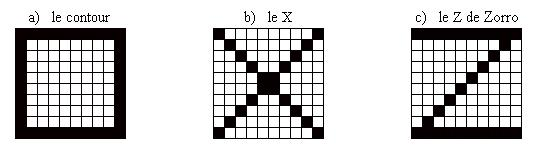
\includegraphics[width=0.7\textwidth]{image/tab2d-ex-oxz}
		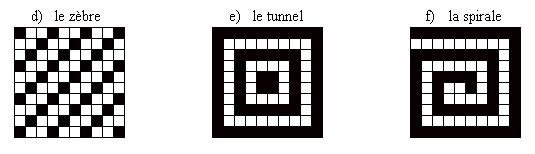
\includegraphics[width=0.7\textwidth]{image/tab2d-ex-zts}
		\end{center}
		
		Notes
		\begin{itemize}
		\item 
			Le zèbre doit toujours présenter des lignes
			obliques et parallèles, quelle que soit la taille.
		\item
			La spirale est un véritable défi
			et vous est donné comme exercice facultatif.
			Ne le faites pas si vous êtes en retard.
		\end{itemize}
	\end{Exercice}

	\begin{Solution}
		\begin{algo}
                  \Algo{pinceauZebre}{\Par{tab\InOut}{\Array{n $\times$ n}{entiers}}}{}{
                    \Assign{colDepart}{0}\;
                    \Fori[]{lg}{0}{n-1}{
                      \Fori[3]{col}{colDepart}{n-1}{
                        \Assign{tab[lg,col]}{NOIR}\;
                      }
                      \eIf{colDepart > 0 }{
                        \Assign{colDepart}{colDepart - 1}\;

                      }{
                        \Assign{colDepart}{2}\;
                      }

                    }
                  }
                  \Algo{pinceauSpirale}{\Par{tab\InOut}{\Array{n $\times$ n}{entiers}}}{}{
                    \Assign{lg}{0}\;
                    \Assign{col}{0}\;
                    \Assign{dirLg}{0}\;
                    \Assign{dirCol}{1}\;
                    \Assign{fini}{faux}\;
                    \While{NON fini}{
                      \Assign{tab[lg,col]}{NOIR}\;
                      \If{bord(lg,col,dirLg, dirCol) OU noircieDansDeuxCase(tab, lg,col,dirLg,dirCol) }{
                        tournerADroite(dirLg, dirCol)\;
                      }
                      avancer(lg, col, dirLg, dirCol)\;
                      \If{caseNoireADroite(tab,lg,col,dirLg, dirCol) }{
                        \Assign{fini}{vrai}\;

                      }
                    }
                  }
                  \Algo{bord}{\Par{lg, col, dirLg, dirCol}{entiers}}{booléen}{
                    \Assign{tmpLg}{lg}\;
                    \Assign{tmpCol}{col}\;
                    avancer(tmpLg, tmpCol, dirLg, dirCol)\;
                    \Return NON (0 <= tmpCol ET tmpCol < n ET 0 <= tmpLg ET tmpLg < n) \;
                  }
                  \Algo{noircieDansDeuxCase}{\Par{tab, lg, col, dirLg, dirCol}{entiers}}{booléen}{
                    \Assign{tmpLg}{lg}\;
                    \Assign{tmpCol}{col}\;
                    avancer(tmpLg, tmpCol, 2*dirLg, 2*dirCol)\;
                    \Return tab[tmpLg, tmpCol] == NOIR
                    \;
                  }
                \end{algo}
                \begin{algo}
                  \Algo{tournerADroite}{\Par{dirLg\InOut}{entier}, \Par{dirCol\InOut}{entier}}{}{
                    \Assign{dirLg}{dirCol}\;
                    \Assign{dirCol}{-dirLg}\;
                  }
                  \Comment{Tests: tournerADroite(0, 1) = (1, 0)}\;
                  \Comment{tournerADroite(1, 0) = (0, -1)}\;
                  \Comment{tournerADroite(0, -1)= (-1, 0)}\;
                  \Comment{tournerADroite(-1, 0)= (0, 1)}\;
                  \Algo{avancer}{\Par{lg\InOut}{entier}, \Par{col\InOut}{entier}, \Par{dirLg, dirCol}{entiers}}{}{
                    \Assign{lg}{lg + dirLg}\;
                    \Assign{col}{col + dirCol}\;
                  }
                  \Algo{caseNoireADroite}{\Par{tab, lg, col, dirLg, dirCol}{entiers}}{booléen}{
                    \Assign{tmpLg}{lg}\;
                    \Assign{tmpCol}{col}\;
                    \Assign{tmpDirLg}{dirLg}\;
                    \Assign{tmpDirCol}{dirCol}\;
                    tournerADroite(tmpDirLg, tmpDirCol)\;
                    \eIf{NON bord(lg,col, tmpDirLg, tmpDirCol) }{
                      avancer(tmpLg, tmpCol, dirLg, dirCol)\;
                      \Return  tab[tmpLg, tmpCol] = NOIR \;
                    }{
                      \Return  faux \;
                    }
                  }
		\end{algo}
	\end{Solution}
	
	\begin{Exercice}{Exercices sur la complexité}	
		Quelle est la complexité 
		\begin{enumerate}[label=\alph*)]
		\item 
			d’un algorithme de parcours	d'un tableau $n$ x $n$ ?
		\item
			des algorithmes que vous avez écrits pour les exercices :
			"Les nuls", "Tous positifs", "Le carré magique"
			et "Le contour d'un tableau" ?
		\item 
			des algorithmes que vous avez écrits pour résoudre les
			exercices du pinceau ?
		\end{enumerate}
	\end{Exercice}